\documentclass[12pt]{article}

\usepackage{sbc-template}
\usepackage{graphicx,url,hyperref}

\usepackage[brazilian]{babel}
%\usepackage[latin1]{inputenc}
\usepackage[utf8]{inputenc}

\usepackage{listings}
\sloppy

\title{Análise Forense em Pacotes de Dados:\\Captura e Remontagem}

\author{Guilherme de M. M. Taschetto\inst{1}}

\address{Faculdade de Informática -- Pontifícia Universidade \\Católica do Rio Grande do Sul
  (PUCRS)\\Porto Alegre -- RS -- Brazil
}

\begin{document}

\maketitle

\begin{abstract}
  This article presents an introduction to network capture and analysis forensics tools, enlighetning its importance, operation and discurring about its usage implications and results.
\end{abstract}

\begin{resumo}
  Este artigo apresenta uma introdução às ferramentas forenses de captura e análise de rede, salientando a sua importância, a sua forma de funcionamento e discorrendo sobre as implicações do seu uso e de seus resultados.
\end{resumo}

\section{Introdução}

A importância da perícia forense digital cresceu muito nos últimos anos. Através de processos, metodologias e ferramentas, a perícia forense digital é capaz de produzir as evidências e provas necessárias para condenar (ou inocentar) criminosos digitais.

Os 4 passos da análise forense de rede são:

\begin{itemize}
\item Identificar fontes de evidência aceitas pelo sistema legal;
\item Preservar a evidência;
\item Analisar a evidência;
\item Apresentar o resultado da análise.
\end{itemize}

Abordaremos ferramentas para a realização dos passos 2 e 3 da análise forense, as chamadas ferramentas de rede para perícia forense.

O segundo passo (preservar a evidência) consiste na coleta de dados de todos os ativos disponíveis na rede como: IDS, IPS, Servidor de Logs, conexões capturadas por sniffers de rede etc. Após a coleta de evidências, é necessário realizar a análise destes pacotes - terceiro passo da análise forense. Para isto, são utilizadas as ferramentas de análise forense de redes, onde os pacotes capturados serão usados como base para remontar os dados reais das camadas mais altas de aplicação.

Tais dados ajudam ajudam o perito computacional na obtenção de evidências para solução dos casos, fornecendo provas irrefutáveis que serão apresentadas no laudo pericial.

\section{Ferramentas de Captura de Pacotes - Preservando a Evidência}

O \texttt{PCAP} é uma API (Application Programming Interface) para a captura de tráfego de rede. Em sistemas operacionais baseados em Linux, o \texttt{PCAP} pode ser utilizado através da biblioteca \texttt{libpcap}, mantida pelo time de desenvolvedores do TCPDump; já em sistemas Windows, a biblioteca é distribuída por meio da \texttt{WinPCap}, mantida pela Riverbed Tech, principal patrocinador do projeto Wireshark.

O \texttt{PCAP} provê uma forma integrada para realizar a captura e a filtragem inteligente de pacotes de rede, suportando uma imensa gama de protocolos, sejam abertos ou proprietários. Além disso, a biblioteca provê a funcionalidade de persistência destes pacotes capturados em arquivos, o que atende o objetivo do segundo passo da análise forense de rede: preservar a evidência.

A API do \texttt{PCAP} é escrita em linguagem C, possuindo wrappers para diversas linguagens e frameworks populares, como C++, Java, Ruby, Haskell, Perl, OCaml, TCL, Python, GoLang, entre outros.

\subsection{Wireshark}

O Wireshark\footnote{https://www.wireshark.org/} é um analisador de pacotes multi-plataforma, grátis e de código-fonte aberto. Possui uma interface gráfica bastante amigável e de fácil utilização com vários recursos integrados, desenvolvida utilizando o toolkit GTK+ a API \texttt{PCAP} para realizar a captura e filtragem de pacotes. Também existe uma versão baseada em linhas de comando chamada TShark (menos famosa).

O Wireshark permite a operação no modo promíscuo, onde todo o tráfego da rede visível pela interface é capturada, e não somente tráfego direcionado aos endereços locais ou de broadcast/multicast. Entretanto, o modo promíscuo tem sua utilidade ceifada em redes que utilizam switches, uma vez que o tráfego dos pacotes já é direcionado.

\begin{figure}[ht]
    \centering
    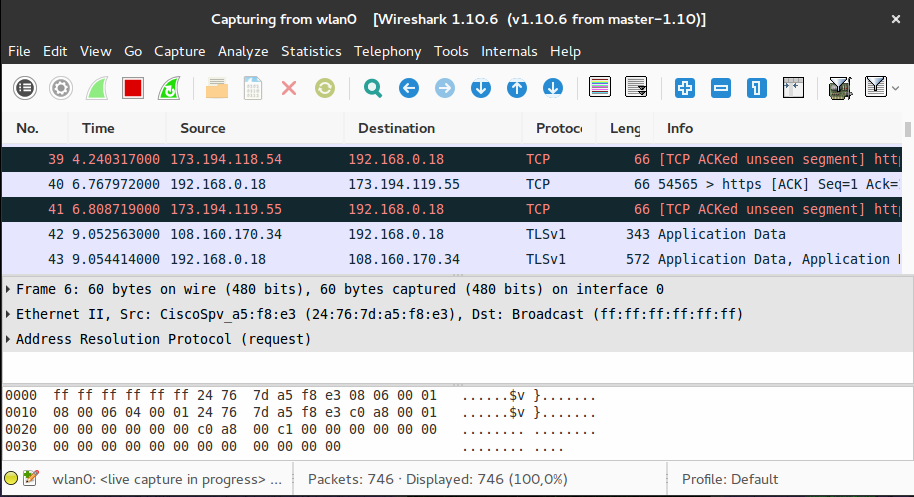
\includegraphics[scale=0.4]{img/wireshark.png}
    \caption{Wireshark, o \"predador\" de pacotes.}
    \label{fig:wireshark}
\end{figure}

\subsection{tcpdump}

O tcpdump\footnote{http://www.tcpdump.org/} é um analisador de pacotes operado por linha de comando. No modo padrão de operação, o tcpdupmp imprime o conteúdo de pacotes no terminal, sejam pacotes capturados ao vivo ou proveniente de arquivos de pacotes armazenados.

Assim como o Wireshark, o tcpdump também pode operar no modo promíscuo.

\textbf{Exemplo de utilização:} \texttt{tcpdump -i wlan0 -A tcp port http -w capture.pcap}

\textbf{Explicação:} capture todos os pacotes HTTP (TCP) na interface wlan0 e salve-os no arquivo capture.pcap.

\begin{figure}[ht]
    \centering
    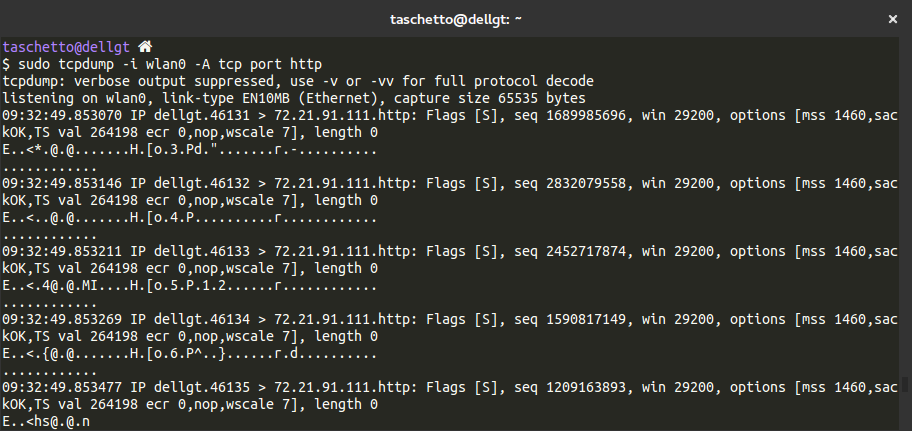
\includegraphics[scale=0.4]{img/tcpdump.png}
    \caption{tcpdump furiosamente capturando pacotes HTTP.}
    \label{fig:tcpdump}
\end{figure}

\subsection{ngrep}

O ngrep\footnote{http://ngrep.sourceforge.net/} é uma ferramenta bastante parecida com o tcpdump, com o diferencial de possuir a capacidade de filtrar pacotes aplicando expressões regulares nos respectivos payloads.

\textbf{Exemplo de utilização:} \texttt{ngrep -l -q -d wlan0 -i "\^{}GET | \^{}POST" \ tcp and port 80 -O capture.pcap}

\textbf{Explicação:} capture todos os pacotes na porta TCP 80 (HTTP) na interface wlan0 que sejam do tipo GET ou POST e salve-os no arquivo capture.pcap.

\begin{figure}[ht]
    \centering
    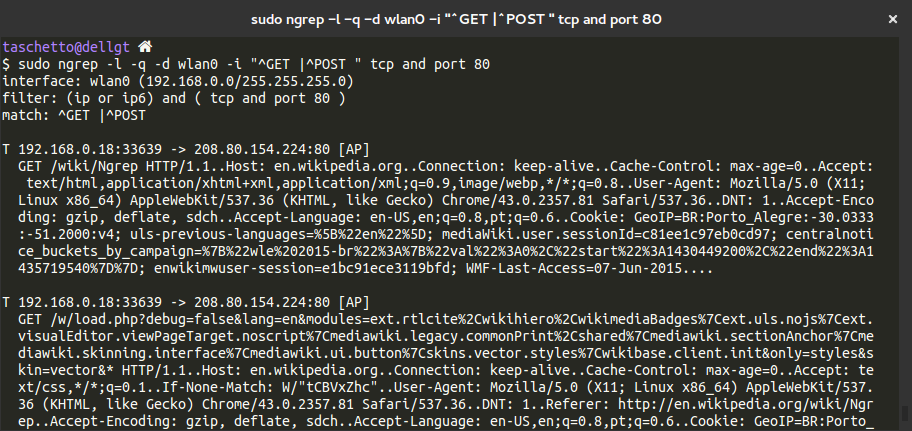
\includegraphics[scale=0.4]{img/ngrep.png}
    \caption{O ngrep é capaz filtrar pacotes de forma sagaz utilizando expressões regulares.}
    \label{fig:ngrep}
\end{figure}

\section{Ferramentas de Análise Forense de Redes - Analisando a Evidência}

Ferramentas de Análise Forense de Redes (Network Forensic Analysis Tool, NFAT) normalmente realizam análises à partir de arquivos \texttt{PCAP}. Em arquivos \texttt{PCAP} são armazenados fluxos de comunicação de rede de diversos protocolos. Ao analisar estes arquivos, as ferramentas NFAT conseguem extrair os dados das comunicações. Por exemplo:

\begin{itemize}
  \item Requisições e páginas HTML (com JS e CSS) sobre o protocolo HTTP;
  \item E-mails sobre os protocolos POP, SMTP e IMAP;
  \item Conversas telefônicas sobre o protocolo SIP;
  \item Entre diversas outros protocolos, como DNS, ARP, SIP, FTP, TFTP etc.
\end{itemize}

Porém não há mágica: não há como remontar os dados trocados em comunicações seguras (criptografadas), porém é possível identificar diversas informações da comunicação em si - por exemplo, endereços físicos e lógicos das partes envolvidas.

Além disso é importante salientar que as ferramentas NFAT não são ferramentas de análise e captura de protocolos de rede, e sim ferramentas de análise forense de redes. Embora algumas até possuam o recurso de capturar pacotes, este não é um requisito para considerar a ferramenta NFAT, tampouco é o foco de seus recursos.

\subsection{Xplico}

O Xplico é uma ferramenta NFAT open-source cujo objetivo é extrair dados contidos em arquivos de capturas de pacotes (formato \texttt{PCAP}). O Xplico é distribuído sob a GNU General Public License e alguns scripts sob a Creative Commons Attribution-NonCommercial-ShareAlike 3.0 Unported (CC BY-NC-SA 3.0) License.

As principais características do Xplico são:

\begin{itemize}
  \item Protocolos suportados: HTTP, SMTP, POP, IMAP, SIP, FB, chat, FTP, MSN, IRC, Telnet etc;\footnote{A tabela completa de protocolos suportados pode ser encontrada em http://www.xplico.org/status.}
  \item Identificação de Protocolo Independente de Porta (PIPI) para cada protocolo de aplicação;
  \item Multithreading;
  \item Cada dado remontado pelo Xplico é associado à um arquivo XML contendo todo o fluxo de pacotes correspondentes ao dado remontado;
  \item Remontagem TCP com verificação de ACK para qualquer pacote;
  \item Lookup de DNS reverso;
  \item Sem limite de tamanhos de dados de entrada;
  \item Suporte a IPv4 e IPv6;
  \item Modularidade. Cada componente do Xplico é modular.
\end{itemize}

O Xplico pode ser instalado e executado em qualquer distribuição Linux. Além disso, o projeto hospeda uma versão de demonstração na web suportando arquivos PCAP com no máximo 5 MB. A versão de demonstração pode ser acessada em \href{http://demo.xplico.org/}{http://demo.xplico.org/}.

\subsection{CapAnalysis}

O CapAnalysis é uma ferramenta NFAT web proprietária que também extrai dados à partir de arquivos \texttt{PCAP}. Diferentemente do Xplico, o CapAnalysis proprietário e, portanto, sua licença de uso deve ser paga.

As principais características do CapAnalysis são:

\begin{itemize}
  \item Suporte aos protocolos mais utilizados diariamente no mundo inteiro;
  \item Remontagem TCP;
  \item Filtro avançado de fluxos \texttt{PCAP};
  \item Inspeção profunda e detalhada de pacotes;
  \item Geolocalização.
\end{itemize}

Assim como o Xplico, o CapAnalysis pode ser instalado e executado em qualquer distribuição Linux. Também conta com uma versão de demonstração online, não informando se há limite para o tamanho do arquivo \texttt{PCAP}. A versão de demonstração pode ser acessada em \href{http://pcap.capanalysis.net/}{http://pcap.capanalysis.net/}.

\section{Estudo de Caso: Xplico}

Como o foco aqui é a análise forense dos pacotes, foi gerado um arquivo \texttt{PCAP} realizando uma captura de alguns segundos através do Wireshark. Durante a captura foram acessadas páginas web não criptografadas, realizadas sincronias utilizando o Dropbox, entre outras operações de rede menos significativas. À partir deste arquivo gerado foi possível extrair diversas informações no Xplico.

\begin{figure}[ht]
    \centering
    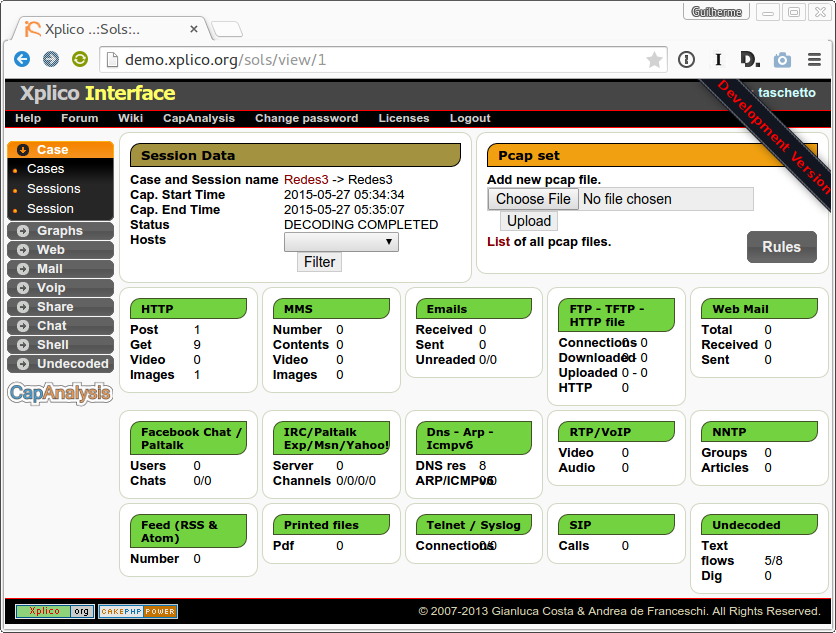
\includegraphics[scale=0.4]{img/2.png}
    \caption{Resumo da Análise}
    \label{fig:report}
\end{figure}

\begin{figure}[ht]
    \centering
    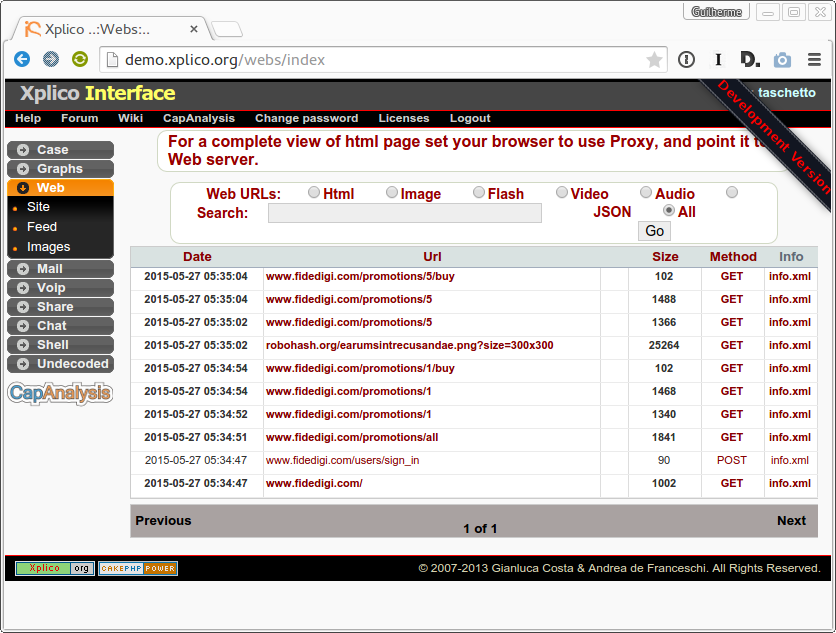
\includegraphics[scale=0.4]{img/1.png}
    \caption{Requisições HTTP}
    \label{fig:http}
\end{figure}

\begin{figure}[ht]
    \centering
    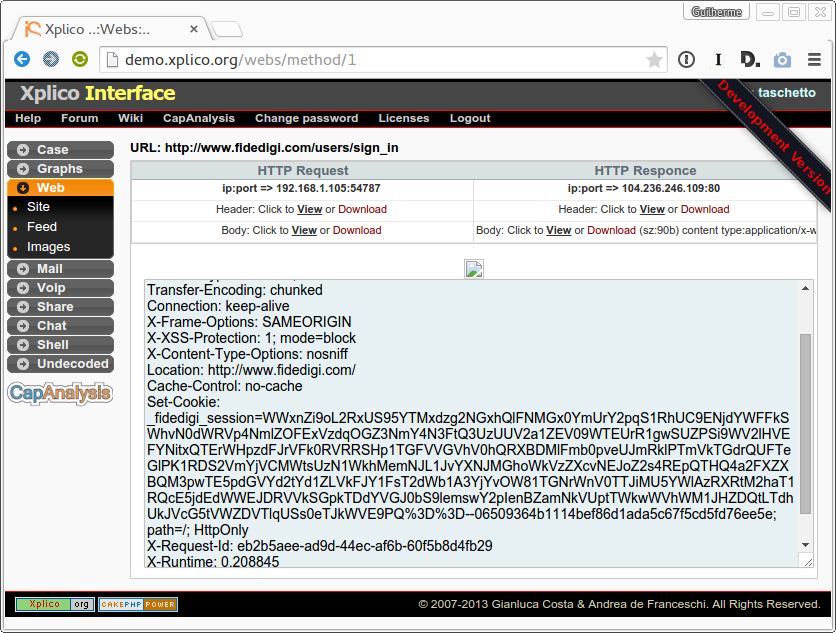
\includegraphics[scale=0.4]{img/3.png}
    \caption{Detalhe do HTTP POST contendo o cookie de sessão}
    \label{fig:cookie}
\end{figure}

\begin{figure}[ht]
    \centering
    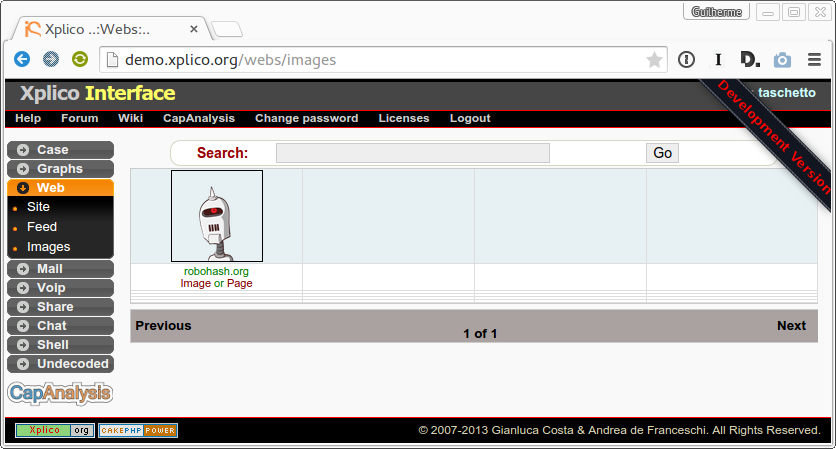
\includegraphics[scale=0.4]{img/4.png}
    \caption{Imagem Recuperada}
    \label{fig:imagem}
\end{figure}

\section{Conclusão}

Após a pesquisa e o estudo de ferramentas NFAT, fica evidente a sua relevância e aplicação na computação forense moderna. Executar ferramentas de captura em modo promíscuo e capturar todo o tráfego de uma rede é uma tarefa trivial. Ser capaz de filtrar e analisar de forma rápida e simples estes dados capturados é de grande importância, seja em investigações públicas como em investigações corporativas. Por exemplo, poder-se-ia identificar usuários acessando conteúdos indevidos na empresa (redes sociais, pornografia, etc) ou até mesmo buscar por consumidores de pedofilia ao analisar o tráfego em pontos estratégicos em WANs.

Entretanto, considero estas ferramentas uma faca de dois gumes: ao mesmo tempo que auxilia na identificação e condenação de infratores e criminosos, também afeta a privacidade dos bons usuários das redes, que não cometem crimes e tem suas informações acessadas muitas vezes sem o seu consentimento.

\nocite{*}
\bibliographystyle{sbc}
\bibliography{sbc-template}

\end{document}
